\documentclass{anpet}

\usepackage{graphicx,import}
\usepackage{booktabs}
\usepackage[english, portuguese]{babel}
\usepackage{csquotes}
\usepackage{hanging}
\usepackage{subfigure}
\usepackage{multirow}
\usepackage{siunitx}
\usepackage[hidelinks]{hyperref}
\usepackage{float}
\sisetup{output-decimal-marker = {,}}
%\usepackage{natbib}
%\bibliographystyle{ieeetr}

\addbibresource{ref.bib} %adicione o nome do arquivo com as referencias

\title{COMO PREPARAR UM TRABALHO PARA APRESENTAÇÃO \protect\\ NO CONGRESSO DE PESQUISA E ENSINO EM TRANSPORTES}

%quebras de linha dentro de nomes de instituições precisam ser protegidas (usar \protect\\ ao invés de \\), se não bagunça a centralização
%O estilo da ANPET é omisso sobre a possibilidade de mais de uma instituição. Não diz se cada instituição deve ficar logo depois os autores da instituição, ou se todas as instituições devem ficar no final. Escolhi a segunda opção. Pra mudar precisaria re-escrever algumas coisas na classe.<<
%\author{}
\author{José Reynaldo A. Setti}
\author{Manoel Henrique A. Sória}
\affil{Universidade de São Paulo \protect\\Escola de Engenharia de São Carlos}

\date{\today}
\begin{document}
\maketitle

\begin{resumo}
Este texto contém instruções para a preparação de trabalhos para os Congressos de Pesquisa e Ensino em Transportes e considerações gerais a respeito da produção de artigos técnicos e científicos. A formatação usada no texto segue rigorosamente as normas de preparação de trabalhos, à exceção do número de páginas; os autores podem dirimir eventuais dúvidas observando o formato do texto. A estrutura do texto segue a recomendada para os trabalhos: resumo e "abstract", introdução, desenvolvimento do texto, considerações finais, agradecimentos, referências bibliográficas e endereço dos autores. O texto também procura esclarecer como o processo de seleção de trabalhos é conduzido.
\end{resumo}

\begin{abstract}
This paper provides information for authors who plan to submit papers to the \textit{Congressos de Pesquisa e Ensino em Transportes} along with guidelines for writing scientific and technical papers. This text is itself formatted in strict accordance with manuscript specifications, with the exception of length; thus, the text serves as a model that can be used to clarify potential doubts. The organization of this text also follows the structure recommended for papers: abstract, introduction, development of the text, concluding remarks, acknowledgments, references and authors’ address. Finally, the criteria and process used to review and select papers for inclusion in this conference are also described.
\end{abstract}
\footnotesize
%\renewcommand{\baselinestretch}{1}

\normalsize
%\renewcommand{\baselinestretch}{1}

\section{INTRODUÇÃO} {
Este artigo é endereçado aos autores que pretendam escrever textos para serem apresentados nos Congressos de Pesquisa e Ensino em Transportes, que são organizados anualmente pela ANPET. Por este motivo, contém recomendações específicas das normas de publicação e preparação de artigos adotadas por esta organização. A despeito disto, sua leitura pode ser útil a autores preparando textos para serem publicados em veículos técnicos ou científicos como revistas, anais e similares.

Muitas das recomendações aqui apresentadas baseiam-se na experiência adquirida pelos autores escrevendo seus próprios trabalhos, orientando dissertações e teses e ao participar de comissões científicas e corpos editoriais de congressos e revistas, analisando trabalhos preparados por colegas de profissão. Uma outra parte dos conselhos aqui apresentados provém de autores que se dedicaram a tratar da difícil arte de escrever trabalhos científicos. Em virtude do pequeno espaço disponível este artigo só aborda as questões mais relevantes, e de modo abreviado. As recomendações aqui contidas, além de expressar a opinião dos autores, estão restritas no espaço e no tempo: refletem costumes da região (quiçá do país...) e dos tempos atuais.

Aborda-se o processo de análise e seleção de trabalhos adotados pelo comitê científico do Congresso de Pesquisa e Ensino em Transportes, procurando mostrar aos potenciais autores alguns pontos que podem determinar se o seu trabalho vai ser aceito ou recusado. As normas adotadas para elaboração de trabalhos são também apresentadas.
}

\section{NORMAS GERAIS PARA ELABORAÇÃO DE TRABALHOS}
As normas gerais que regem a elaboração de trabalhos para o Congresso de Pesquisa e Ensino em Transportes devem ser estritamente respeitadas pelos autores. Os trabalhos podem estar escritos em português, espanhol ou inglês. A data limite para recebimento dos trabalhos é definida nas comunicações de chamada de trabalho e deve ser respeitada rigorosamente, a fim de não prejudicar o cronograma de produção dos anais e o processo de solicitação de auxílio junto às entidades financiadoras. Trabalhos não poderão ser enviados fora do prazo, pois o sistema de submissão eletrônica será desabilitado após encerramento do prazo de submissão.

\subsection{Categorias de trabalhos}
Os trabalhos apresentados nos congressos da ANPET podem ser de três categorias diferentes: artigos, comunicações técnicas e relatórios de teses e dissertações em andamento. Os autores devem definir cuidadosamente em qual categoria o trabalho melhor se insere, pois os critérios de julgamento usados pelo comitê científico são diferentes para cada uma das três categorias. A escolha da categoria não deve ser feita em função do número de páginas do trabalho, mas sim em função das suas características, que estão descritas a seguir. Durante o processo de seleção o comitê científico não transfere trabalhos de uma categoria para outra; um dos critérios para rejeição é a incompatibilidade do trabalho com a categoria escolhida pelos autores.

\subsubsection{Artigos}
A categoria artigos engloba trabalhos inéditos de natureza técnico-científica. Esses trabalhos devem ter características comumente presentes em artigos científicos, tais como: rigor técnico e científico, contribuição para o estado da arte ou da prática, clareza, validade do método usado e das conclusões apresentadas, etc. Devem ter entre 8 e 12 páginas, que contenham todos os seus elementos (resumo, "abstract", corpo do artigo, bibliografia, figuras, tabelas etc.). Veja, em outras seções deste texto, algumas orientações para a preparação de artigos para os congressos da ANPET.

\subsubsection{Comunicações técnicas}
Na categoria comunicações técnicas incluem-se trabalhos inéditos que relatam, por exemplo, projetos e resultados de aplicações de técnicas inovadoras etc. Na sua avaliação, um aspecto significativo é a contribuição para a disseminação da aplicação de técnicas inovadoras na solução de problemas de transportes. As comunicações técnicas devem ter entre 4 e 8 páginas, devem apresentar um resumo no mesmo formato do apresentado nos artigos e não devem conter "abstract". As orientações para a preparação de artigos devem ser também levadas em consideração no preparo de comunicações técnicas.

\subsubsection{Relatórios de teses e dissertações em andamento}
Esta categoria foi criada para permitir que alunos de mestrado e doutorado possam apresentar seus projetos de pesquisa e tirar proveito da presença de pesquisadores de diversos centros no congresso, que podem fazer sugestões e discutir os resultados já obtidos. Devem ser necessariamente escritos em co-autoria pelo aluno e seu orientador. Como este relatório trata de uma pesquisa em andamento, os autores, na apresentação do trabalho no congresso, devem abordar novos resultados e avanço obtidos no período decorrido entre a preparação do trabalho e o congresso. Os relatórios devem estar contidos, no máximo, em 4 páginas, que devem apresentar, no mínimo, a proposta da pesquisa, uma revisão bibliográfica sintética sobre o assunto da proposta e uma descrição suficientemente detalhada do método usado; resultados intermediários também devem ser apresentados, caso já existam. Os relatórios de teses e dissertações em andamento devem apresentar resumo, mas não "abstract". Como o propósito dos relatórios é discutir pesquisas em andamento, dá-se preferência à apresentação e trabalhos que apresentam pesquisas mais avançadas, em relação àqueles que tratam de pesquisas em estágio ainda incipiente.

\subsubsection{Relatórios de pesquisa de iniciação científica}
Esta categoria contempla trabalhos de pesquisa de iniciação científica realizadas por alunos de graduação, e devem ser submetidos pelo aluno em co-autoria com o(s) orientador(es). Os relatórios de pesquisa de iniciação científica devem ser apresentados em 2 páginas e conter, no mínimo, resumo, objetivo do trabalho, método utilizado, principais resultados obtidos, conclusões do estudo e referências bibliográficas. Os relatórios não devem apresentar "abstract", e as demais orientações para a preparação de artigos também são válidas para a elaboração desses trabalhos.

\section{FORMATO GERAL DOS TRABALHOS}
Somente trabalhos completos devem ser enviados para o processo de análise e seleção. Os anais do congresso serão produzidos a partir da versão final dos trabalhos selecionados, da forma como preparado pelos autores. Por isso, é importante que as regras para formato geral dos trabalhos sejam seguidas rigorosamente, a fim de que exista uma harmonia entre os artigos publicados nos anais.

O processo de seleção de trabalhos é o conhecido por "double-blind", no qual os autores desconhecem a identidade dos avaliadores e os avaliadores desconhecem a autoria do trabalho. Assim sendo, os autores deverão enviar uma versão completa do texto do trabalho para uso no processo de seleção sem que esta contenha a identificação dos autores. Os trabalhos selecionados deverão ser revisados e os comentários e sugestões dos avaliadores deverão ser incorporados à versão final, que será usada para a confecção dos anais do congresso.
A única diferença de formato entre a versão submetida para avaliação e a versão final de trabalhos aceitos é a ausência da identificação dos autores e instituições a que pertencem na versão submetida para avaliação.

O trabalho deve ter um formato similar a este documento, que foi preparado de acordo com as instruções para os autores. A \autoref{fig:formato1Pag} ilustra o formato da primeira página da versão final de trabalhos aceitos para o congresso. Na versão do trabalho enviada para avaliação, as linhas correspondentes à identificação dos autores e instituições devem ser suprimidas. Na preparação dos trabalhos, os autores devem observar rigorosamente as seguintes características:

\begin{itemize}
\item papel tamanho A4;

\item páginas sem cabeçalhos ("headers"), rodapés ("footers"), numeração de páginas ou logotipos de empresas, universidades ou centros de pesquisa;

\item a margem direita deve ter 2 cm, as três margens restantes devem  ter 3 cm;

\item letras do tipo Times Roman, tamanho 12, para o texto principal, e Times Roman tamanho 10, para o texto e título do resumo, \textit{abstract} e bibliografia;

\item espaçamento simples entre linhas;

\item os parágrafos começam na margem esquerda do texto, estando separados entre si por uma linha em branco;

\begin{figure}[H]
  \begin{center}
    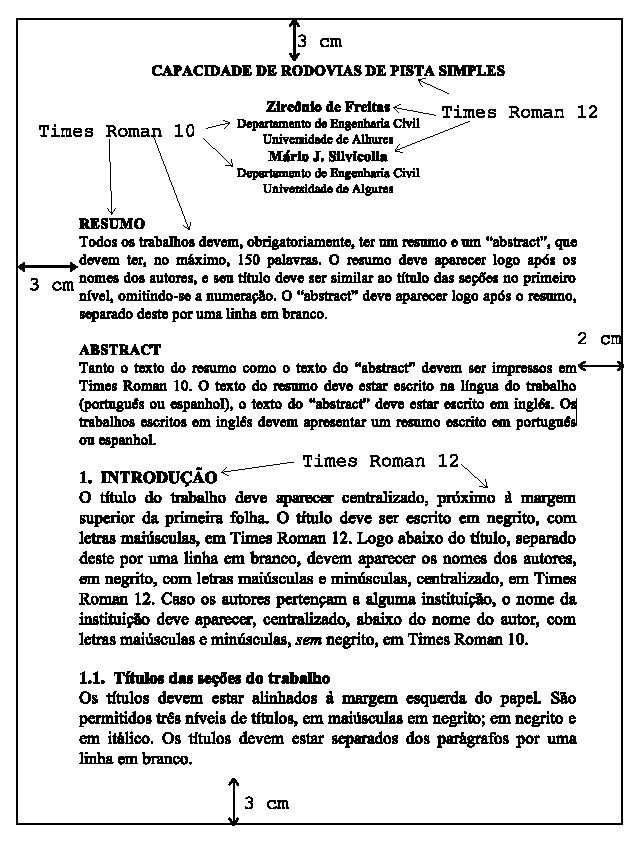
\includegraphics{Figuras/Figura_1.eps}
    \caption{Formato geral da primeira página do trabalho}
    \label{fig:formato1Pag}
  \end{center}
\end{figure}

\item os títulos de seções do trabalho devem estar separados do parágrafo precedente por uma linha em branco. Devem estar numerados (a menos do resumo, "abstract" e das referências bibliográficas) e alinhados pela margem esquerda. As seções podem ser numeradas em até
três níveis;

\item os títulos no primeiro nível devem aparecer em maiúsculas, em negrito, com letras tamanho 12 pontos, com a numeração 1., 2., 3., etc., conforme mostrado na \autoref{fig:formato1Pag};

\item os títulos no segundo nível devem aparecer em negrito, em maiúsculas e minúsculas, com letras tamanho 12 pontos, com a numeração 1.1., 1.2. etc., como ilustrado na \autoref{fig:formato1Pag};

\item os títulos no terceiro nível devem aparecer em itálico, em maiúsculas e minúsculas, com letras tamanho 12 pontos, com numeração 1.1.1., 1.1.2. etc;

\item os títulos do resumo, "abstract" e referências bibliográficas devem ser similares aos títulos de seções no primeiro nível, omitindo-se a numeração e com letras tamanho Times Roman 10;

\item nunca use notas de rodapé ou no final do texto; se a informação for imprescindível, ela deve ser incluída no texto do trabalho;

\item nunca use notas de rodapé para referências bibliográficas;

\item palavras destacadas devem aparecer em itálico, nunca em negrito ou sublinhadas. Termos estrangeiros devem aparecer entre aspas ou em itálico;

\item o título do trabalho deve aparecer centralizado, próximo à margem superior da primeira folha. O título deve ser escrito em negrito, com letras maiúsculas, em Times Roman 12. Logo abaixo do título, separado deste por uma linha em branco, devem estar os nomes dos autores, em negrito, com letras maiúsculas e minúsculas, centralizado, em Times Roman 12. Caso os autores pertençam a alguma instituição, o nome da instituição deve aparecer, centralizado, abaixo do nome do autor, com letras maiúsculas e minúsculas, \textit{sem} negrito, em Times Roman 10;

\item o endereço dos autores, incluindo-se o endereço de E-mail (caso exista), deve ser colocado após as referências bibliográficas, no final do trabalho. Na cópia usada na seleção, o endereço dos autores não deve aparecer, para preservar a anonimidade dos autores (não usar a cor branca para os caracteres de identificação pois isso permite a recuperação da informação no formato PDF);

\item os artigos devem, obrigatoriamente, ter um resumo e um “abstract” com, no máximo, 150 palavras cada. O resumo deve estar logo após os nomes dos autores. O “abstract” deve estar logo após o resumo, separado deste por uma linha em branco;

\item as comunicações técnicas, os relatórios de teses e dissertações, e os relatórios de pesquisa de iniciação científica devem, obrigatoriamente, ter um resumo com, no máximo 150 palavras; o resumo deve estar logo após os nomes dos autores; essas categorias de trabalho não devem apresentar “abstract”;

\item o texto do resumo deve estar escrito na língua do trabalho (português ou espanhol), o texto do “abstract” deve estar escrito em inglês. Os trabalhos escritos em inglês devem apresentar um resumo escrito em português ou espanhol;

\item não repita o título do trabalho e os nomes dos autores na segunda página do trabalho. Não faça uma página exclusiva para o resumo e “abstract”. A ilustração da \autoref{fig:formato1Pag} mostra o formato da primeira página do trabalho;

\item as referências bibliográficas devem estar logo após o texto do trabalho, em Times Roman 10. Veja as instruções específicas para as citações bibliográficas no texto e para a preparação da lista de referências bibliográficas;

\item caso exista uma seção de agradecimentos, ela deve aparecer entre as conclusões e as referências bibliográficas. O seu título deve ser similar aos títulos das seções no segundo nível (maiúsculas e minúsculas em negrito), omitindo-se a numeração. O tamanho das letras deve ser Times Roman 10, para o título e texto da seção.

\end{itemize}

Terminado o processo seletivo, os autores de trabalhos selecionados para apresentação e publicação nos anais deverão preparar uma versão final do trabalho, na qual estejam incorporados os comentários e sugestões dos avaliadores e apareça a identificação dos autores e suas respectivas filiações.

Tanto a versão para revisão como a versão definitiva deverão ser enviadas através do sistema eletrônico da ANPET, no endereço:

\begin{center}
\href{<http://www.anpet.org.br/ssat>}{\textit{http://www.anpet.org.br/ssat}}
\end{center}

\section{Equações, tabelas e figuras}
As equações, figuras e tabelas devem estar inseridas no texto, ser escritas com o mesmo tipo e tamanho de letra usado no texto do trabalho (Times Roman 12) e numeradas sequencialmente. Os números devem aparecer entre parênteses, alinhados pela margem direita do papel, estando as equações centralizadas, como indicado no exemplo:
\begin{equation}
  R = c_1G + C_2GV + C_a AV^2 + 10Gi
  \label{eq:res_total}
\end{equation}
\begin{condições}
  R & resistência total [N];\\
  c_1 & constante;\\
  G & peso bruto total combinado [kN];\\
  c_2 & constante;\\
  V & velocidade [km/h];\\
  c_a & coeficiente de penetração aerodinâmica;\\
  A & seção transversal do veículo [m\textsuperscript{2}]; e\\
  i & declividade da rampa [m/100 m].
\end{condições}

Não deixar linhas em branco entre a equação e os parágrafos que a precedem e antecedem, como pode ser visto no exemplo da \autoref{eq:res_total}.

Para as tabelas, usa-se o mesmo tipo de letra do texto, mas faculta-se aos autores o uso de letras num tamanho menor, desde que este tamanho não seja inferior a Times Roman 9, pois a tabela deve ser perfeitamente legível quando reduzida.

As tabelas devem ser elaboradas com espaçamento simples e numeradas sequencialmente, aparecendo centralizadas na folha. Todas terão um título auto-explanatório. O título é limitado a duas linhas e deve aparecer acima da tabela, sem estar separado dela. Se o título tiver apenas uma linha, ele deve ser centralizado; caso contrário, será alinhado pela margem esquerda do papel. Use linhas verticais apenas nos casos em que sua ausência pode tornar mais difícil a leitura da tabela. Não use negrito para os títulos das colunas, nem use sombras para ressaltar linhas ou colunas da tabela.

\begin{table}[H]
\centering
\caption{Relação volume-velocidade medida no local}
\label{tab:relacao_vol_vel}
\begin{tabular}{S[table-format=4.0] S[table-format=4.0]}
\toprule
\multicolumn{1}{c}{Volume (veic/h)} & \multicolumn{1}{c}{Velocidade (km/h)}\\
\midrule
1852 &  43\\
1576 & 101\\
800  & 115\\
820  & 122\\ 
\bottomrule
\end{tabular}
\end{table}
O título das tabelas deve iniciar-se pela palavra \textbf{Tabela}, em negrito, o número da tabela (também em negrito), dois pontos (:), seguidos pelo texto do título, como mostrado no exemplo da \autoref{tab:relacao_vol_vel}. As tabelas devem estar separadas do parágrafo que a antecede por uma linha em branco. O parágrafo que aparece após uma tabela deve estar separado dela por uma linha em branco.

As figuras (em preto e branco ou coloridas) serão numeradas sequencialmente e terão título auto-explanaório. O formato dos títulos das figuras é similar ao das tabelas, substituindo-se apenas a palavra \textbf{Tabela} por \textbf{Figura} e invertendo-se a sua posição em relação à figura: o título deve aparecer abaixo da figura e não acima dela. As figuras devem estar separadas do texto por uma linha em branco, como no caso das tabelas, e devem ficar centralizadas na página. Para os gráficos serão usadas letras do mesmo tipo do texto (Times Roman) ficando facultado aos autores usar um tamanho menor que Times Roman 12, desde que as letras não tenham tamanho inferior a 9 pontos. A \autoref{fig:graf_vel_vol} ilustra como uma figura deve aparecer no trabalho.

\begin{figure}[H]
  \begin{center}
    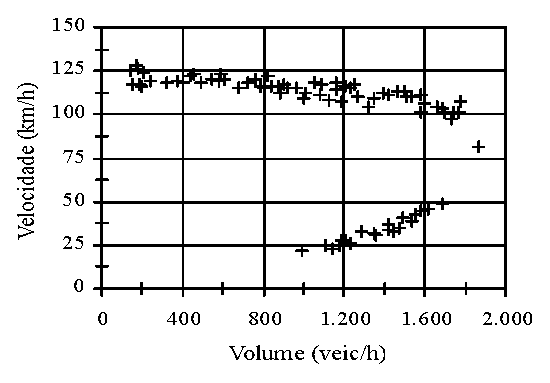
\includegraphics{Figuras/Figura_2.eps}
    \caption{Variação da velocidade média com o volume de tráfego}
    \label{fig:graf_vel_vol}
  \end{center}
\end{figure}

As equações devem, obrigatoriamente, fazer parte do arquivo que contém o texto do trabalho.As figuras e tabelas devem também estar contidas no mesmo arquivo do texto do trabalho. Caso isto não seja possível, os autores devem entrar em contato com o comitê organizador do congresso para instruções sobre como agir.

\section{REFERÊNCIAS BIBLIOGRÁFICAS}

As referências bibliográficas são obrigatórias para as contribuições propostas na categoria artigo, na categoria relatório de tese ou dissertação em andamento, e na categoria relatórios de pesquisa de iniciação científica e opcionais na categoria comunicação técnica. No texto, as citações deverão ser referenciadas pelo(s) sobrenome(s) do(s) autor(es) e o ano da publicação, tudo entre parênteses. Desta forma têm-se: (Beltrano, 1994), para um único autor; (Fulano e Beltrano, 1987), para dois autores; e para mais de dois autores, (Fulano et al., 1990). Nos casos em que o nome do autor faz parte do texto, apenas o ano é colocado entre parênteses, logo após o nome do autor: Fulano (1994).

Nos casos onde existem duas referências publicadas no mesmo ano, estas devem aparecer como (Fulano e Beltrano, 1994a) e (Fulano e Beltrano, 1994b). Se as referências forem relativas a dois trabalhos do mesmo autor, não é preciso repetir o nome do autor, bastando repetir o ano (Sicrano, 1988, 1992, 1994b). Às vezes, é necessário fazer referência a diversos trabalhos no conjunto de parênteses; nesses casos, usa-se ponto e vírgula para separar trabalhos de autores diferentes (Fulano, 1987; Beltrano, 1994a, 1994b; Sicrano et al., 1992).

No final do texto do artigo haverá uma lista com as referências bibliográficas, em ordem alfabética dos sobrenomes dos autores. Cada referência deve aparecer num parágrafo, cuja primeira linha deverá estar alinhada pela margem esquerda da página e cujas linhas subsequentes deverão estar recuadas de 1 cm. Não deixe nenhuma linha em branco entre referências. Use o mesmo tipo de letra do texto do trabalho (Times Roman), tamanho 10. Inclua na lista apenas as referências que são citadas no texto; não esqueça de incluir na lista todas as referências citadas no trabalho.

Uma referência inicia-se com o sobrenome do autor, uma vírgula e suas iniciais. Caso exista um segundo autor, após as iniciais do primeiro autor aparece a conjunção \textit{e}, as iniciais do segundo autor e seu sobrenome. Se existirem mais de dois autores, coloque o nome de todos os autores. Após o(s) nome(s) do(s) autor(es), coloque o ano de publicação, entre parênteses. Note que não se usa ponto nem traço para separar o ano e o título da referência. O título e os itens restantes da referência vão depender do tipo de trabalho referenciado. Veja os exemplos, para melhor compreensão.

No caso de artigos publicados em periódicos, o nome do artigo deve ser escrito em maiúsculas e minúsculas (conforme as regras gramaticais da língua portuguesa) e o nome do periódico deve aparecer em itálico. Não deixe de colocar o volume, o número e as páginas inicial e final, na forma v. 23, n. 5, p. 1025–1029. Veja \textcite{hong1996estimating}, nas referências bibliográficas ao final deste texto, para verificar como um artigo de periódico deve aparecer naquela lista. 

Para artigos publicados em anais de conferências, o título do artigo é escrito em maiúsculas e minúsculas e o título dos anais aparece em itálico. \textcite{fonseca1997transporte}, na lista de referências bibliográficas ao final deste texto, mostra como um artigo publicado em anais de congressos científicos deve aparecer na lista de referências bibliográficas. Não se esqueça de colocar o volume e as páginas inicial e final na referência.

No caso de livros, o título deve aparecer em maiúsculas e minúsculas, em itálico. \textcite{rosenberg1976logica}, na lista de referências bibliográficas, ilustra como um livro aparece na lista de referências bibliográficas. Num capítulo de livro, o autor do capítulo aparece em primeiro lugar, seguido pelo ano da publicação entre parênteses e o título do capítulo. A seguir, aparece a palavra In:, em itálico, o(s) nome(s) do(s) editor(es), seguidos da palavra (eds.), entre parênteses e em itálico, do título do livro, em itálico, da nome da editora e do local de edição. \textcite{Jonhson1990DiscreteChoice} mostra como um capítulo de livro deve aparecer na lista de referências.

No caso de publicações sem autor, o nome ou a sigla da instituição responsável pela publicação deve aparecer no lugar do nome do autor. \textcite{GEIPOT1995}, na lista de referências, é uma referência sem autor.

% \section{O texto escrito}

\begin{acknowledgements}
Os autores agradecem as sugestões recebidas de diversos colegas, que permitiram aprimorar o texto e eliminar diversas inconsistências. Caso haja necessidade de se fazer referência a alguma instituição de apoio à pesquisa, deve-se fazê-lo sob a forma de um agradecimento, nesta parte do texto.
\end{acknowledgements}

\footnotesize
\printbibliography 

\vfill


\hrulefill\\
Renan Artur Lopes Eccel (renan.eccel@gmail.com) \\
Rodrigo Castelan Carlson (rodrigo.carlson@ufsc.br)\\
Programa de Pós-graduação em Engenharia de Automação e Sistemas, Universidade Federal de Santa Catarina\\
Florianópolis, SC, 88040-900, Brasil


\end{document}

